%  !TeX  root  =  user_guide.tex

\chapter{Plugin di QGIS}\label{sec:plugins}\index{plugins}

% when the revision of a section has been finalized,
% comment out the following line:
% \updatedisclaimer

QGIS è stato progettato con un'architettura estensibile tramite plugin. 
Ciò permette di aggiungere nuove caratteristiche e funzioni
all'applicazione. Molte delle caratteristiche in QGIS sono in effetti implementate come plugin di
base \textbf{Core} o \textbf{Esterni}.\index{plugin!tipi} 

\begin{itemize}[label=--]
\item I \textbf{Plugin Core} sono mantenuti dal team di sviluppo di QGIS e fanno automaticamente 
parte di ogni distribuzione QGIS.
Sono scritti in uno dei due seguenti linguaggi: C++ o Python.
Ulteriori informazioni riguardanti i plugin core sono disponibili nella sezione \ref{sec:core_plugins}.
\item I \textbf{Plugin Esterni} sono scritti in Python.
Sono memorizzati in archivi esterni e mantenuti dai singoli autori.
Possono essere aggiunti a QGIS usando l'\filename{Installatore di plugin Python}.
Ulteriori informazioni riguardanti i plugin esterni sono disponibili nella Sezione \ref{sec:load_external_plugin}.
\end{itemize}

\section{Gestione dei plugin}\label{sec:managing_plugins}
\index{plugin!gestione} 

La gestione dei plugin consiste nella loro abilitazione o disabilitazione usando il \filename{Gestore plugin}.
I plugin esterni devono prima essere installati usando l'\filename{Installatore di plugin Python}.
Per attivare/&disattivare i plugin esterni, una volta installati, si usa il \filename{Gestore plugin}.

\subsection{Abilitare un Plugin Core}\label{sec:load_core_plugin} 

L'abilitazione di un Plugin Core si ottiene dal menu principale \mainmenuopt{Plugins} \arrow 
\dropmenuopttwo{mActionShowPluginManager}{Gestione plugins...}.\index{plugin!gestione}

\begin{figure}[ht]
   \centering
   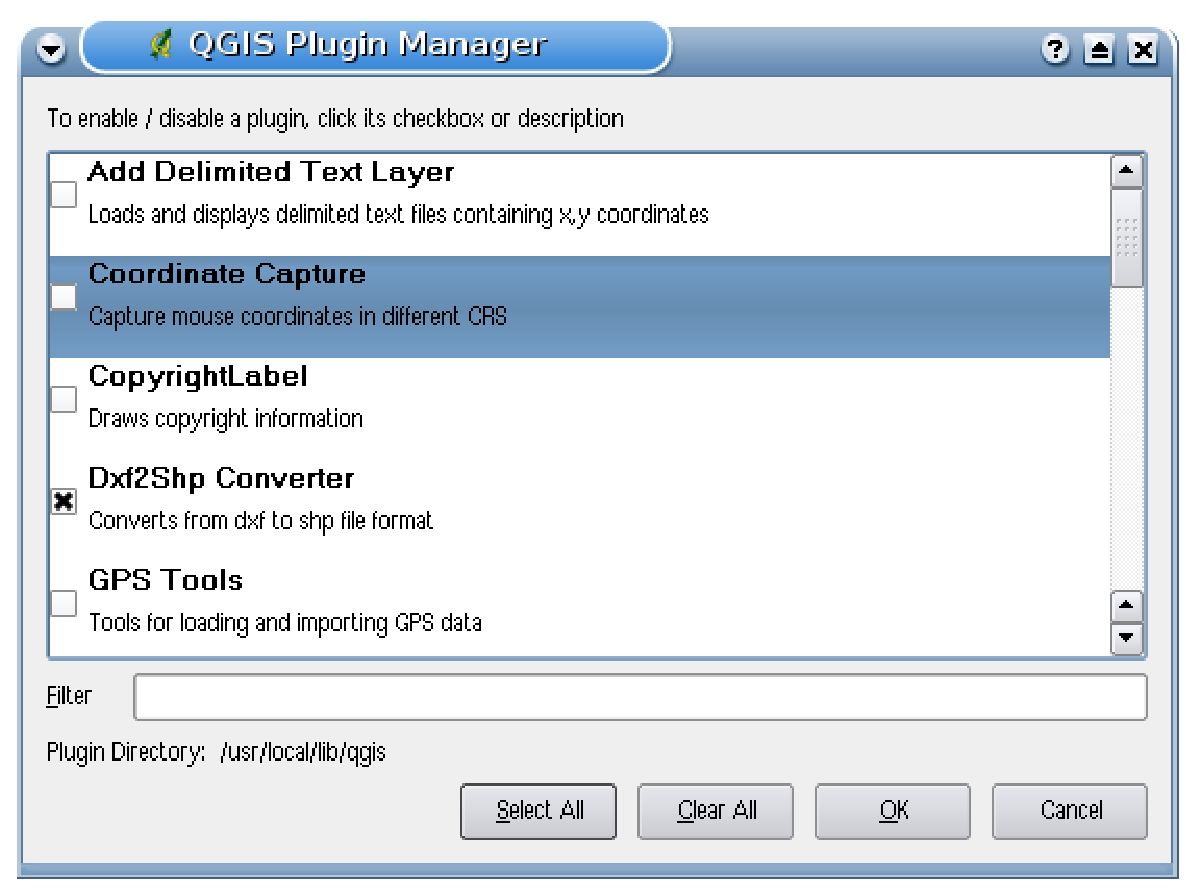
\includegraphics[clip=true, width=12cm]{pluginmanager}
   \caption{Gestore plugin QGIS \nixcaption}\label{fig:pluginmanager}\smallskip
\end{figure}

Il \filename{Gestore QGIS Plugin} elenca tutti i plugin disponibili e il loro stato (abilitato o disabilitato).
Sono disponibili tutti i plugin Core e tutti i plugin Esterni che sono stati aggiunti usando 
l'\filename{Installatore di plugin Python} (Sezione \ref{sec:load_external_plugin}).
I plugin abilitati hanno una casella di controllo attivata sulla sinistra del loro nome: 
per abilitare un plugin, quindi, abilitare la casella di controllo e cliccare su \button{OK}.
La Figura \ref{fig:pluginmanager} mostra la finestra di dialogo del gestore dei plugin.

Lo stato dei plugin, attivo/disattivo, viene memorizzato quanto si termina una sessione di QGIS, in modo tale 
che al successivo riavvio, i plugin vengano automaticamente caricati.

\begin{Tip}\caption{\textsc{Blocco dei plugin}}\index{blocchi}
Se QGIS si blocca all'avvio, la colpa potrebbe essere di un plugin. 
È possibile disabilitare il caricamento dei plugin modificando il file delle impostazioni 
(Sezione \ref{subsec:gui_options}). 
Una volta individuate le impostazioni dei plugin, bisogna impostare il valore di 
ognuno su "false" in modo da impedirne il caricamento. \nix {Per esempio per disabilitare il plugin 
Testo delimitato, la modifica da effettuare sul file \$HOME/.config/QuantumGIS/qgis.conf 
in Linux dovrebbe apparire così: \usertext {Add Delimited Text Layer=false}.} \normalfont 
Eseguire l'operazione per tutti i plugin della sezione, avviare successivamente QGIS ed 
aggiungere i plugin uno alla volta tramite il \filename{Gestore plugin} per determinare quale stia causando 
il problema.
\end{Tip}

\subsection{Caricamento di un plugin esterno}\label{sec:load_external_plugin} 

I plugin Esterni sono scritti in Python e risiedono negli archivi
'Ufficiali' di QGIS, in quelli 'Utenti-Contributori' oppure in vari archivi esterni 
mantenuti dai singoli autori. 
Tutti gli archivi sono disponibili nell'\filename{Installatore plugin python}, 
raggiungibile da
\dropmenuopttwo{plugin_installer}{Recupero Plugin Python...}.

Documentazione dettagliata, versione minima di QGIS richiesta, pagina web, autori ed 
altro sono forniti con i plugin stessi e non inclusi in questo manuale.
\footnote{Aggiornamenti dei plugin Core potrebbero essere forniti in archivi esterni.}
\footnote{fTools, Mapserver Export e l'Installatore dei plugin sono plugin Python, ma 
sono anche parte del codice di QGIS, quindi vengono automaticamente caricati e abilitati 
nel gestore di plugin (Sezione~\ref{sec:load_external_plugin}).}

Al momento attuale sono disponibili oltre 120 plugin distribuiti tramite 13 archivi.
Alcuni di questi plugin offrono funzionalità comuni richieste da molti utenti 
(es. visualizzare e modificare dati Open Street Map 
o caricare layer di Google Map), mentre altri plugin offrono funzionalità molto 
specialistiche (es. Calculate economic pipe diameters for water supply networks).

È oltremodo intuitivo cercare plugin esterni tramite parola chiave, scegliere un 
archivio o impostare un filtro in funzione dello stato dei plugin (installato 
o non installato). La ricerca e il filtraggio vengono fatti nel gestore dei plugin 
(Figura~\ref{fig:plugininstaller}).

\begin{Tip} \caption{\textsc{Aggiungere ulteriori archivi}}
Per aggiungere un archivio 'Utente contributore' e/o archivi di autori, aprire 
l'installatore di plugin (\mainmenuopt{Plugins} \arrow \dropmenuopttwo{plugin_installer}{Recupero Plugin Python...}),
andare alla scheda \tab{Repository} e cliccare su \button{Aggiungi repository di terze parti}.
Per aggiungere/modificare/eliminare un archivio cliccare rispettivamente su \button{Aggiungi...}, 
\button{Modifica...}, \button{Elimina}.
\end{Tip}

Per integrare un plugin esterno in QGIS è necessario:

\begin{itemize}[label=--]
\item Scaricare il plugin dall'archivio tramite l'\filename{Installatore Plugin Python} 
(Sezione \ref{sec:python_plugin_installer}): il plugin verrà aggiunto alla lista
dei plugin disponibili nel \filename{Gestore Plugin} e caricato automaticamente.
\end{itemize}

\subsection{Uso dell'installatore di Plugin Python}\index{plugin!installazione}\label{sec:python_plugin_installer}
\index{plugin!installatore plugin Python}\index{plugin!aggiornamento}

\begin{figure}[ht]
   \centering
   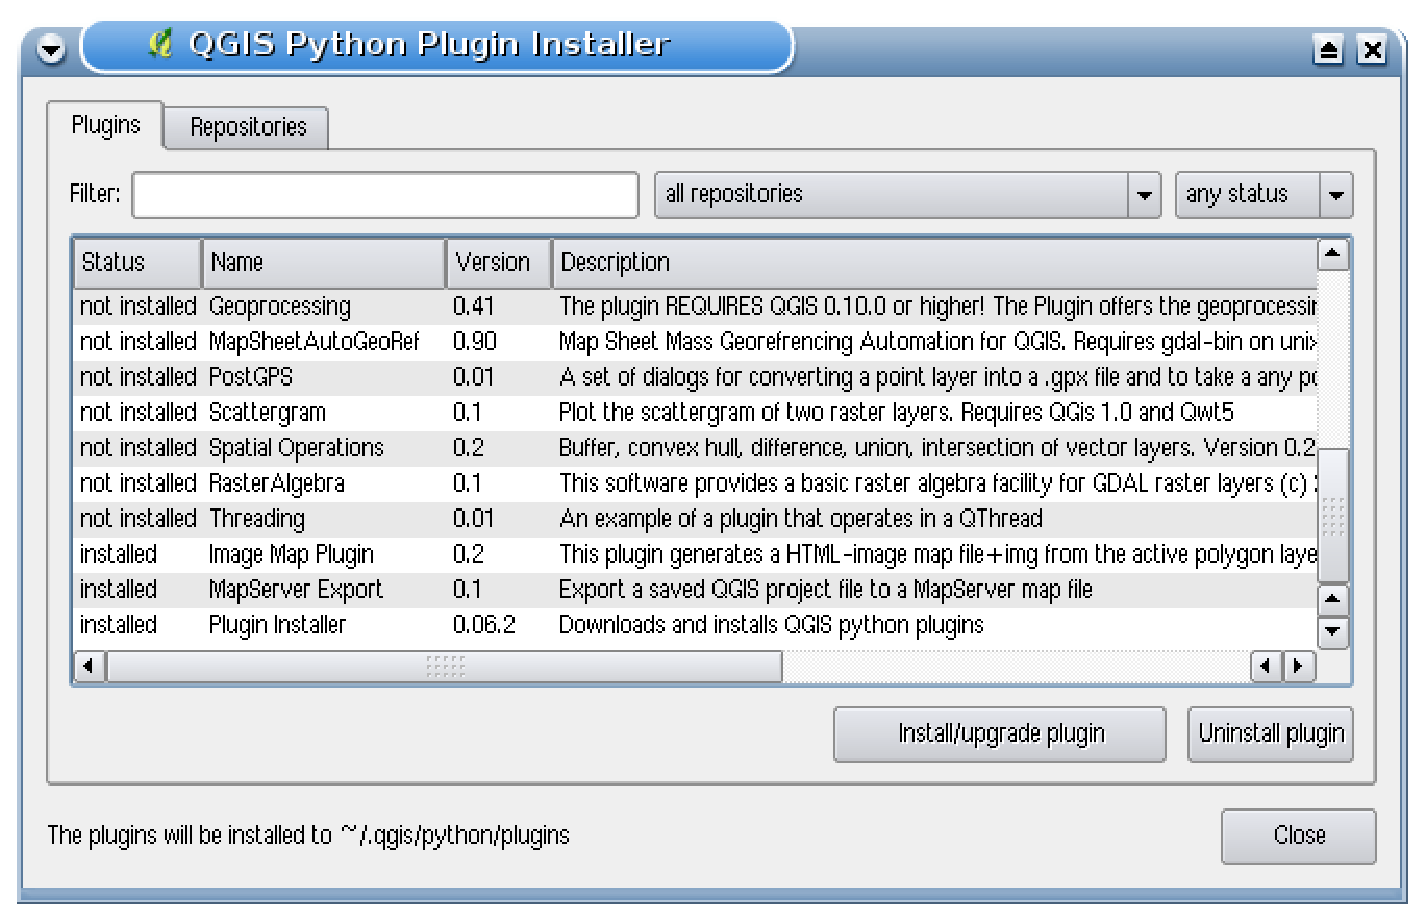
\includegraphics[clip=true, width=12cm]{plugininstaller}
   \caption{Installazione di plugin Esterni Python \nixcaption}\label{fig:plugininstaller}\smallskip
\end{figure}

Per scaricare ed installare un plugin python esterno, cliccare su \mainmenuopt{Plugins} \arrow \dropmenuopttwo{plugin_installer}
{Recupero Plugin Python...}: si aprirà la finestra di dialogo \filename{Installatore plugin python} 
(Figura \ref{fig:plugininstaller}) con la scheda \tab{Plugin} contenente la lista sia di tutti i plugin python 
disponibili negli archivi remoti sia di quelli installati. Ogni plugin può essere:
\begin{itemize}
\item \textbf{non installato} - significa che il plugin è disponibile nell'archivio remoto, ma non ancora installato. 
Per installarlo, selezionarlo dalla lista e cliccare su  \button{Installa plugin}.
\item \textbf{nuovo} - significa che il plugin è nuovo tra quelli disponibili nell'archivio.
\item \textbf{installato} - il plugin è installato. Se è anche disponibile in qualsiasi archivio remoto il pulsante 
\button{Reinstalla plugin} è abilitato. Se la versione disponibile in remoto è più vecchia di quella installata, 
appare invece il pulsante \button{Downgrade plugin}.
\item \textbf{aggiornabile} - il plugin è installato, ma è disponibile in una versione più recente. 
Il pulsante \button{Aggiorna plugin} è abilitato.
\item \textbf{non valido} - il plugin è installato, ma è inutilizzabile. La ragione è spiegata nella descrizione del plugin.
\end{itemize}

\minisec{Scheda Plugin}

Per installare un plugin, selezionarlo dalla lista e cliccare su \button{Installa plugin}. Il plugin è attivato ed 
installato nella sua propria directory.

\begin{itemize}[label=--]
\item \nix{Linux ed altri unix}:\\
./share/qgis/python/plugins \\
/home/\$USERNAME/.qgis/python/plugins
\item \osx{Mac OS X}:\\
./Contents/MacOS/share/qgis/python/plugins \\
/Users/\$USERNAME/.qgis/python/plugins
\item \win{Windows}:\\
C:\textbackslash Program Files\textbackslash QGIS\textbackslash
python\textbackslash plugins \\
C:\textbackslash Documents and Settings\textbackslash\$USERNAME\textbackslash
.qgis\textbackslash python\textbackslash plugins
\end{itemize}

Se l'installazione va a buon fine, compare un messaggio di conferma. 

Se l'installazione fallisce ne viene indicata la ragione. I problemi più frequenti sono correlati a errori di 
connessione e/o moduli Python mancanti. Nel primo caso basta attendere e riprovare in un secondo momento, 
nel secondo è necessario installare nel sistema operativo i moduli Python mancanti. \nix{In Linux, i moduli 
più richiesti dovrebbero essere disponibili nel gestore dei pacchetti}. \win{Per istruzioni sull'installazione in 
Windows, visitare la pagine web del modulo}. Se si usa un proxy, può essere necessario configurarlo in
\mainmenuopt{Modifica} \arrow \dropmenuopttwo{mActionOptions}{Opzioni} (Gnome, OSX)
o \mainmenuopt{Impostazioni} \arrow \dropmenuopttwo{mActionOptions}{Opzioni} (KDE, Windows), scheda \tab{Rete}.

Il pulsante \button{Disinstalla il plugin} è abilitato solo se il plugin selezionato è installato e non è un plugin Core. 
Da notare che se si è installato un aggiornamento di un plugin Core, si può sempre disinstallare tale 
aggiornamento con il pulsante \button{Disinstalla il plugin} e ritornare alla versione contenuta nel pacchetto di 
installazione di Quantum GIS, ma il plugin non può essere disinstallato.

\minisec{Scheda Repository}

La scheda \tab{Repository} contiene una lista di archivi di plugin disponibili per l'installazione. 
Come impostazione predefinita viene usato solamente l'archivio ufficiale di QGIS. 
Si possono aggiungere archivi messi a disposizione dagli utenti, incluso l'archivio centrale "QGIS Contributed Repository" 
ed altri archivi esterni, usando il pulsante \button{Aggiungi repository di terze parti}. Questi archivi contengono un gran 
numero di plugin non mantenuti dal Team di Sviluppo di QGIS, pertanto quest'ultimo non se può assumere la responsabilità.
Si può anche gestire la lista dei plugin manualmente, cioè aggiungere, rimuovere o editare le singole voci. 
È possibile disabilitare temporaneamente un particolare archivio usando il pulsante \button{Modifica...}.

\minisec{Scheda Opzioni}

Nella scheda \tab{Opzioni} si possono configurare le impostazioni dell'\filename{Installatore di plugin}. 
La casella di controllo \checkbox{Controlla aggiornamenti all'avvio} indica a QGIS di cercare automaticamente aggiornamenti 
di plugin e novità. Se questa opzione è abilitata, tutti i repository elencati e abilitati nel 
nella scheda \tab{Repository} vengono controllati ogni volta che il programma viene avviato. 
È possibile modificare la frequenza di controllo degli aggiornamenti usando il menu a cascata: sono disponibili le opzioni
una volta al giorno e una volta al mese. Se è disponibile un nuovo plugin o un aggiornamento di quelli 
installati, compare una notifica nella barra di stato. Se la casella di controllo non è attivata, la ricerca di aggiornamenti e 
novità avviene solo quando viene lanciato l'installatore di plugin.

Sebbene l'installatore di plugin sia in grado di gestire porte diverse dalla 80, alcune connessioni internet possono
causare degli errori nel tentativo di controllare automaticamente gli aggiornamenti. 
In questo caso, può esser visibile durante l'intera sessione di QGIS un indicatore \textit{Looking for new plugins...} 
nella barra di stato che può causare il blocco del programma alla chiusura.
Per aggirare il problema, disattivare gli aggiornamenti automatici.

Inoltre, è possibile specificare il tipo di plugin da elencare nell' \filename{Installatore di plugin}. 
Sotto \textit{Plugin disponibili}, si può specificare:

\begin{itemize}[label=--]
\item Mostra solo plugin provenienti da repository ufficiali,
\item Mostra tutti i plugin esclusi quelli marcati come sperimentali,
\item Mostra tutti i plugin, compresi quelli marcati come sperimentali.
\end{itemize}

\begin{Tip}
 \caption{\textsc{Utilizzo dei plugin sperimentali}}
I plugin Sperimentali non sono generalmente adatti al lavoro produttivo. Questi plugin sono in fase prematura di sviluppo e 
sono da considerare 'incompleti' o quali 'idee concettuali'. Il team di sviluppo di QGIS sconsiglia l'installazione di 
questi plugin, a meno che non si intenda usarli per attività di test.
\end{Tip}

\subsection{Fornitori di dati}\index{data provider}

I 'Fornitori dati' sono plugin speciali che danno accesso ad un archivio di dati. Per default, QGIS supporta i layer PostGIS
e gli archivi di dati su disco supportati dalla libreria GDAL/OGR: un plugin fornitore di dati estende la capacità di 
QGIS di utilizzare altre fonti di dati.

Tali plugin sono registrati automaticamente all'avvio di QGIS. Non sono gestiti dal gestore di plugin, 
ma usati dietro le quinte quando un tipo di dati viene aggiunto come layer in QGIS.

\FloatBarrier
